\section{数据预取策略}

%%%%%%%%%%%%%访问模式+数据预取 张江论文中描述的一些挑战和相关工作%%%%%%%%%%%%%%%%%%%%%%%

%如前所述,
I/O问题是制约大规模科学数据计算性能的一个非常重要的瓶颈,特别是在使用按需载入策略的任务并行中。由于科技的快速发展,处理器的性能得到了极大的提高,其处理速度远远大于I/O设备的访问速度,
这也导致在处理器和存储的性能之间出现了一个巨大的鸿沟。
即使使用了诸如PVFS\parencite{CarnsLRT00}、Lustre\parencite{Cluster02}和GPFS\parencite{SchmuckH02}等并行文件系统,
在处理大规模小的非连续的I/O请求时效率还是比较低。

在大规模流场计算的过程中,I/O速率与计算速率的矛盾典型地重。
我们以流场可视化为例探究数据预取的效率。
流场的模拟是许多计算领域的关键。
随着计算能力的不断提高,模拟得到的流场数据规模越来越大,也越来越复杂。
然而,从最实际的角度来看,用于科学可视化的计算资源通常比用于原始模拟的计算资源要小得多,因此带来了挑战。
也就是说,如何在不需要超级计算机参与的情况下,有效地进行大规模(如TB级别)流场可视化。

针对大规模流场数据的并行可视化,研究者设计了一定的数据管理策略,用于管理数据的存储、载入以及在进程间的转移等,以提高在有限资源下大规模流场可视化的I/O和内存的使用效率。
为了提高数据访问的性能,在任务并行粒子追踪中往往会用到数据预取技术。

\begin{figure}[h]
%\setlength{\abovecaptionskip}{0.05cm} 
%\setlength{\belowcaptionskip}{-0.20cm}
  \centering
  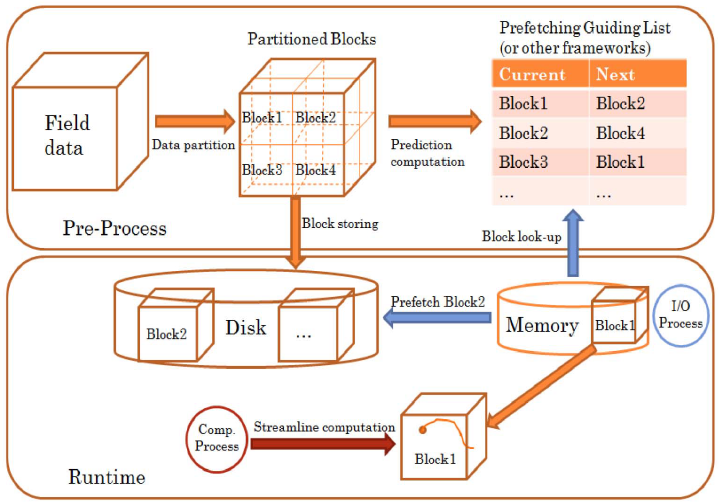
\includegraphics[width=.8\linewidth,keepaspectratio]{image/prefetch/prefetch_pipeline.png}
  \caption{
   数据预取流程图\parencite{Guo2017WL}。
 }
\label{fig:prefetch:prefetch_pipeline}
\end{figure}

数据预取的思想是在载入所需要的数据时,将之后粒子追踪可能访问到的数据也一并提前载入,
这样可以降低I/O操作次数,减少进程因为数据不在内存中而必须等待的时间,
从而提高并行粒子追踪的计算效率。
数据预取的流程图如图\ref{fig:prefetch:prefetch_pipeline}所示。
数据预取的有效性取决于对未来可能访问数据的预测准确度。
在任务并行粒子追踪的应用中,
I/O访问模式往往会被记录下来为数据预取提供依据。 
早在2005年,Rhodes等人\parencite{RhodesTBS05}就将用户访问模式作为先验知识,使用缓存和预取机制来动态提高I/O性能。图\ref{fig:prefetch:initial_prefetch}展示了其基本流程图,其中空间的预取机制成为了链接接迭代的用户访问模式和真实数据存储的重要桥梁。通过发现
迭代的用户访问模式构成的空间中访问的起点,步幅和顺序中的已有规律,可以有助于创建针对迭代进行调整的预取缓存,并进一步地根据真实的存储模型一次性的获取后续需要的文件,提升I/O的效率。接下来本文将总结近年来流场可视化并行粒子追踪过程中,利用不同流场属性特征或I/O访问模式作为先验知识来指导进行数据预取的相关工作。

\begin{figure}[!tb]
%\setlength{\abovecaptionskip}{0.05cm} 
%\setlength{\belowcaptionskip}{-0.20cm}
  \centering
  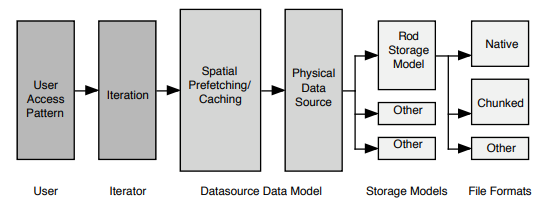
\includegraphics[width=\linewidth,keepaspectratio]{image/prefetch/initial_prefetch_patternbased.png}
  \caption{
   用户访问模式指导的数据预取框架\parencite{RhodesTBS05}。
 }
\label{fig:prefetch:initial_prefetch}
\end{figure}

% 包括访问依赖图和其他更复杂的I/O模式。

\begin{figure}[!tb]
%\setlength{\abovecaptionskip}{0.05cm} 
%\setlength{\belowcaptionskip}{-0.20cm}
  \centering
  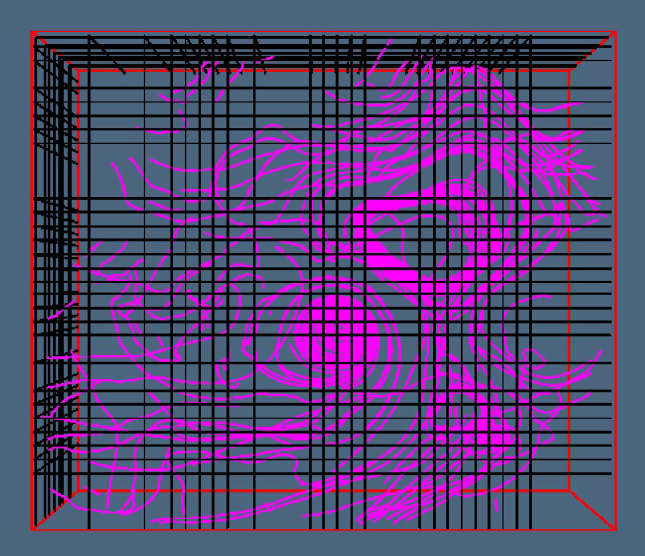
\includegraphics[width=.55\linewidth,keepaspectratio]{image/prefetch/block_partition.png}
  \caption{
   基于流场特征的自适应数据块划分方法效果示例\parencite{Guo2017WL}。其中粉色曲线为随机撒种生成的流线,黑色网格为根据此方法得到的数据块划分结果。
 }
\label{fig:prefetch:block_partition}
\end{figure}

近年来,国防科技大学海洋科学与工程研究院的Guo等人\parencite{Guo2017WL}提出了一种基于流场特征的自适应的数据块划分方法。
对于流场中较为平缓的区域,由于粒子的流向比较一致,采用不同的数据块划分策略对数据预取准确度并没有显著的影响。
而对于流场中的复杂区域,更加细粒度的划分可以更精准地预测粒子在每个数据块的流出方向。
根据上述特点,他们首先由信息熵公式计算出流场内每个区域的复杂度,然后在流场的每个维度上进行不同粒度的划分,如图\ref{fig:prefetch:block_partition}所示。
在不同数据集上的实验结果表明采用此方法可以显著提高数据块的准确预取率及有效预取率,验证了该方法的有效性。

俄亥俄州立大学的可视化小组针对流场可视化中流线和迹线等的计算,
提出了一系列基于数据访问依赖的数据预取方法\parencite{ChenXLS12,ChenNLS12}。
在预处理阶段,他们将数据划分为小块形式,
然后根据粒子追踪的数据访问关系生成数据块之间的访问依赖图(access dependency graph, ADG)。
如图\ref{fig:background:adg-1st}所示,
在访问依赖图中,每个结点代表一个数据块,
结点之间的有向边表示从一个块到另一个块的访问转移关系。
有向边的权重记录了访问转移的概率,即粒子从一个块出发到达另一个块的概率。
他们将这种数据访问依赖图用于文件布局优化,
从而在数据预取过程中帮助精确预测即将可能用到的数据块。
但是,由于访问依赖图的精度和预处理开销对数据块大小和撒种策略等比较敏感,
这些方法比较容易受到参数的影响。

\begin{figure}[!tb]
  \centering
  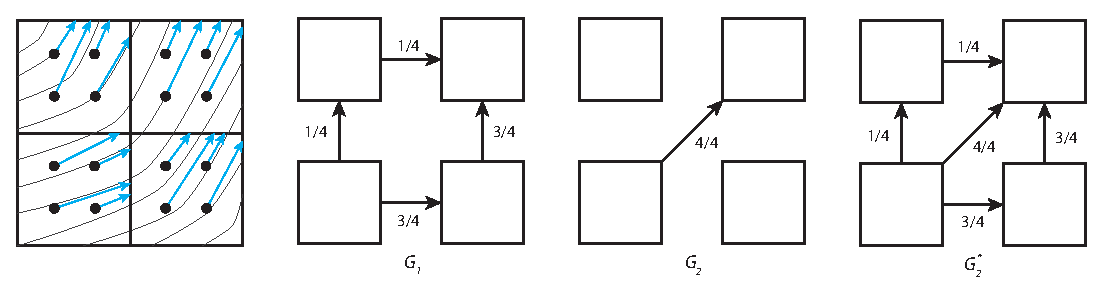
\includegraphics[width=\linewidth]{image/prefetch/adg-1st}
  \caption{
    粒子追踪过程中的访问依赖图\cite{ChenXLS12}。
    图中示例展示了粒子从起始数据块到下一个数据块($G_1$)以及继续到第三个数据块($G_2$)。
    $G_2^*$表示这两个图的混合。
  }
  \label{fig:background:adg-1st}
\end{figure}

首先,粒子的轨迹难以预测。
粒子轨迹本质上是一条积分曲线,这条曲线上的每一采样点位置的计算都依赖于前一点,
其并不像体绘制中那样,给定起始采样点和步长,就可以直接计算出后面每个采样点的位置。 
因此,即使给定了初始粒子的位置,也很难预测其轨迹的走向,
也不知道粒子会访问哪些数据,给数据的管理带来了很大的困难。

而在数据并行中,数据从外存存储组织中,按照初始的划分和分配策略,
被不同的进程载入内存,进行粒子追踪计算。
根据数据块在进程中的分布,粒子在这一过程中会在不同的进程之间交换。
由于粒子追踪计算和数据是紧密耦合的,粒子和数据在并行计算过程中的移动实际上也是紧密相关的。
数据的移动会极大地影响并行粒子追踪的I/O效率和内存使用效率。

另一方面,由于在任务并行粒子追踪过程中一般由进程按需载入数据块,
会导致频繁的I/O开销。已有的工作\parencite{ChenNLS12,ChenXLS12}中研究者们主要将数据进行小块的划分和组织,
通过一个预处理阶段,事先在流场中密集撒种统计粒子在数据块之间的访问先后关系,
生成数据块访问依赖图,然后在并行粒子追踪中使用数据预取技术,
即提前载入可能需要的数据,将I/O操作的时间“隐藏”起来,
减小I/O的开销使得粒子追踪的完成时间集中在计算上。
这里面一般是根据粒子的数据访问模式来进行数据组织,
据此设计数据的访问策略,提高I/O和内存使用效率。
数据的组织是一个预处理过程,需要预先计算数据块之间的访问模式并随原始数据存储管理,
以支持使用数据预取来减少I/O操作。其I/O效率的提高很大程度上取决于数据预取的准确率,
而数据预取的准确率又依赖于对数据的预处理,
这种预处理的复杂性往往和流场的规模和复杂性成正比,
因此目前做法的复杂度都比较高,并且需要比原始数据更大的存储组织空间。

\subsection{一阶访问依赖数据预取}

\begin{figure}[!tb]
  \centering
  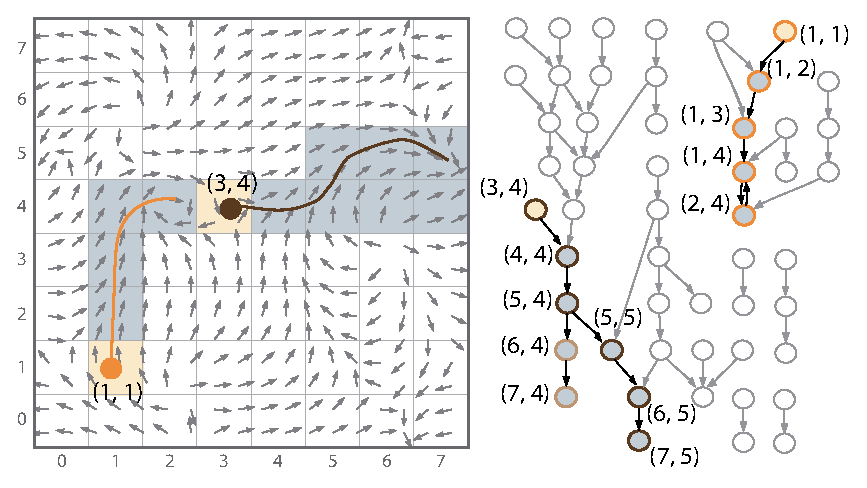
\includegraphics[width=.75\linewidth]{image/prefetch/sparse}
  \caption{
    一阶访问依赖数据预取示意图\parencite{GuoZLLYHMP14}。
  }
  \label{fig:background:sparse}
\end{figure}

在迹线计算中,数据量通常非常巨大,但是其中的迹线计算所需要的数据可能只是其中的一部分。传统的粗粒度的划分可能导致不必要的数据读取。而场线的计算随着粒子的运动具有一定的空间关系,这是由于一些模式导致的。以大规模高维数据可视化为例,对一种稀疏数据管理的方法\cite{guo2014advection}进行分析,该方法首先对数据进行“小块”的细粒度划分,并且使用基于并行键值存储的按需数据管理策略。

在并行计算迹线的过程中,该方法有效平衡了I/O带宽和数据访问请求之间的速度差距。结果表明在任意给定的资源限制下,该方法能够提高数据分析的规模,节约I/O带宽和内存的使用,提高任务并行的并行迹线计算的可扩展性。

\subsection{高阶访问依赖数据预取}

追踪大量的场线。然而,由于巨大的I/O和内存需求,场线的计算是非常昂贵的。特别是I/O开销,往往能占据整个计算时间的90\%。解决I/O负担的一个方法是将数据访问模式结合到场线计算中。数据访问模式由流场数据的特征隐式地决定,其记录了场线轨迹的数据访问情况。可以将其提取出来,并在之后的场线应用中预测数据访问。在已有的方法中,马尔可夫链被用来对数据访问模式进行建模,其思想是通过当前的数据访问预测下一个可能的数据访问。这种访问模式也被称为数据块之间的一阶访问依赖。不过,由于每个数据块可能与多个其他的数据块有访问依赖关系,因此很难得到比较准确和可靠的访问预测。

实际上,除了这种简单的一阶访问模式,在场线追踪中还存在着更为复杂的高阶访问依赖。不同之处就在于高阶访问依赖将历史的数据访问信息也考虑进去了,使之可以得到更为精确的数据访问预测。图\ref{fig:highorder_fig1}给出了一个例子。在图\ref{fig:highorder_fig1}(a)的一阶访问依赖中,数据块0与其三个邻结块1,2,3都有访问依赖关系。因此,对于一个从数据块0出发的粒子, 其下一个要经过的块有三种可能性。而在图\ref{fig:highorder_fig1}(b)的二阶访问依赖中,根据不同的历史访问,下一步要访问的数据块的可能性减小为两个,并且概率更集中。基于此,张江等人提出了一种新颖的基于高阶访问依赖的模型,以高效地计算场线,特别是非定常流场中的迹线。该方法包含两部分,首先通过迹线追踪计算出高阶访问依赖,然后将它们应用到一个并行粒子追踪框架,以证明高阶访问依赖的有效性。

\begin{figure}[!tb]
  \centering
  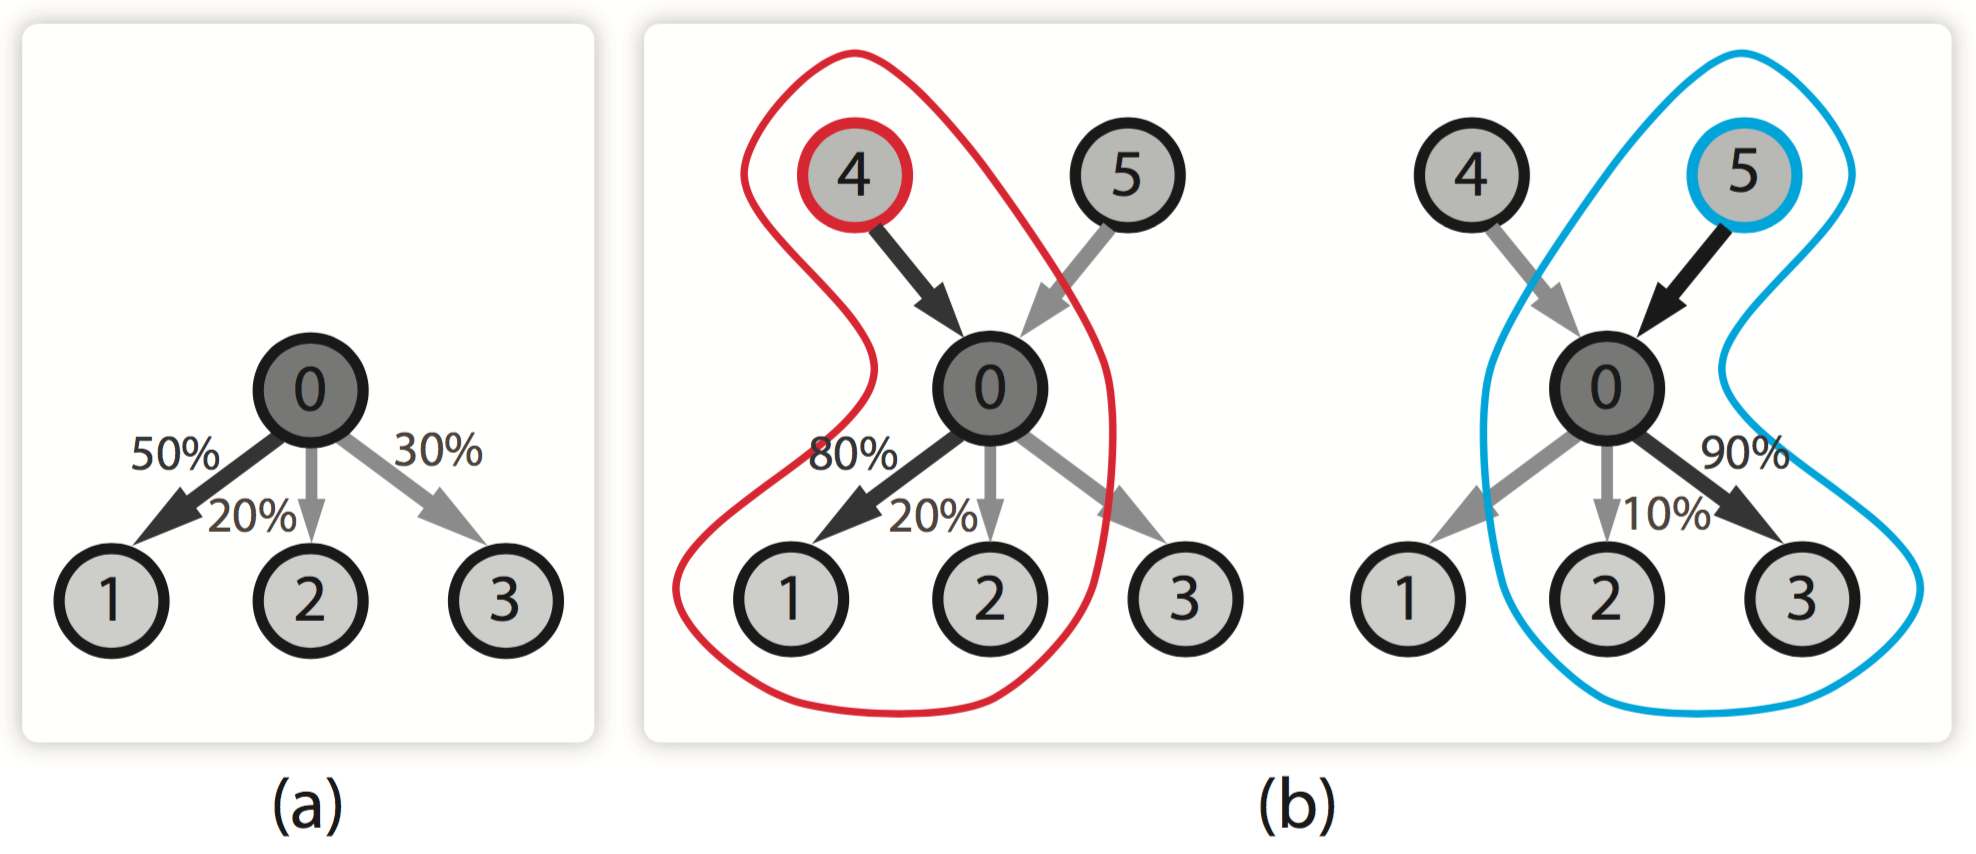
\includegraphics[width=.7\linewidth]{image/prefetch/highorder_fig1.png}
  \caption{
    使用图模型展示的(a)一阶和(b)二阶访问依赖的比较。\parencite{ZhangGY16}
  }
  \label{fig:highorder_fig1}
\end{figure}

与一阶访问依赖相比,在高阶访问依赖模型中,对下一个可能访问的数据块的预测不仅依赖于当前的数据访问,还建立在若干历史数据访问序列上。对于一个m阶访问依赖,有图\ref{fig:highorder_fig2}所示的定义。

\begin{figure}[!tb]
  \centering
  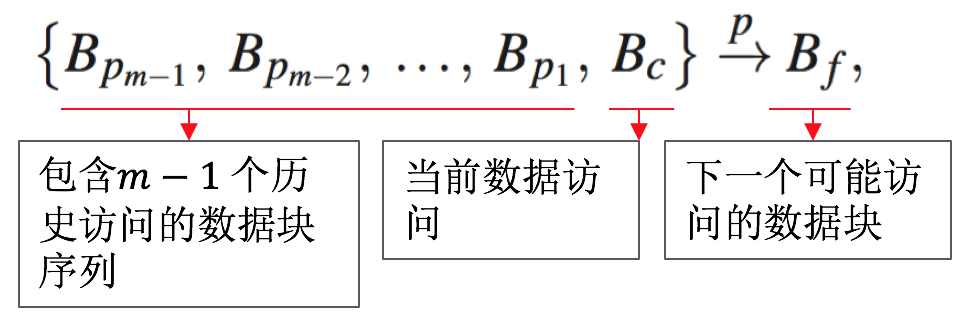
\includegraphics[width=.6\linewidth]{image/prefetch/highorder_fig2.png}
  \caption{
    m阶访问依赖的定义。\parencite{ZhangGY16}
  }
  \label{fig:highorder_fig2}
\end{figure}

为了生成高阶访问依赖,首先需要在数据全域内追踪迹线。整个数据被均匀划分为若干数据块,每个块都包含了各个维度上相等大小的范围,并且使用均匀撒种的方式在不同位置放置粒子。每个粒子从起始位置开始同时正向和反向进行追踪。对应生成的迹线分别叫做正向迹线和反向迹线。为了减小预处理开销,对于正向迹线只追踪它从起始块转移到下一个数据块,而对于反向迹线,其所经过的数据块的数量不能大于指定的阶数。实际上,始于同一个位置的正向和反向迹线可以合并成一条完整的同时包含历史和下一步访问信息的迹线。对这些合并的迹线,除去起始块,对应的反向迹线所访问的数据块可看成是历史访问信息,而对应的正向迹线访问的数据块则是即将可能的访问信息。

对于指定$m (m > 1)$阶的访问依赖,考虑历史访问的数据块序列长度为$m - 1$的所有合并迹线。因为这些迹线的历史访问信息可能仍有不同,因此将它们进一步分组。每组迹线的历史访问信息是相同的,但是下个数据访问可能是不同的。假设下一个访问的数据块共有$n$种可能性,在该方法中,每个关联相同访问历史$B_p$ (序列$B_{p_{m − 1}}, B_{p_{m − 2}}, …, B_{p_1}$的简写)和当前访问$B_c$的下一个可能的数据块$B_{f_i}$都会对应一个高阶访问依赖。其对应的访问转移概率$p_i$定义为下一个访问该数据块的所有迹线数量与访问所有可能数据块的迹线总数的比值。该过程示意图如图\ref{fig:lstm_fig2}所示。为了充分利用所生成的迹线, 计算所有阶数低于该指定值的访问依赖。这样只要一轮预处理计算,就可以满足使用不同阶访问依赖的迹线实际应用。在本节的部分,除非特别指出,所说的某高阶访问依赖都是这种“累积”的访问依赖。

\begin{figure}[!tb]
  \centering
  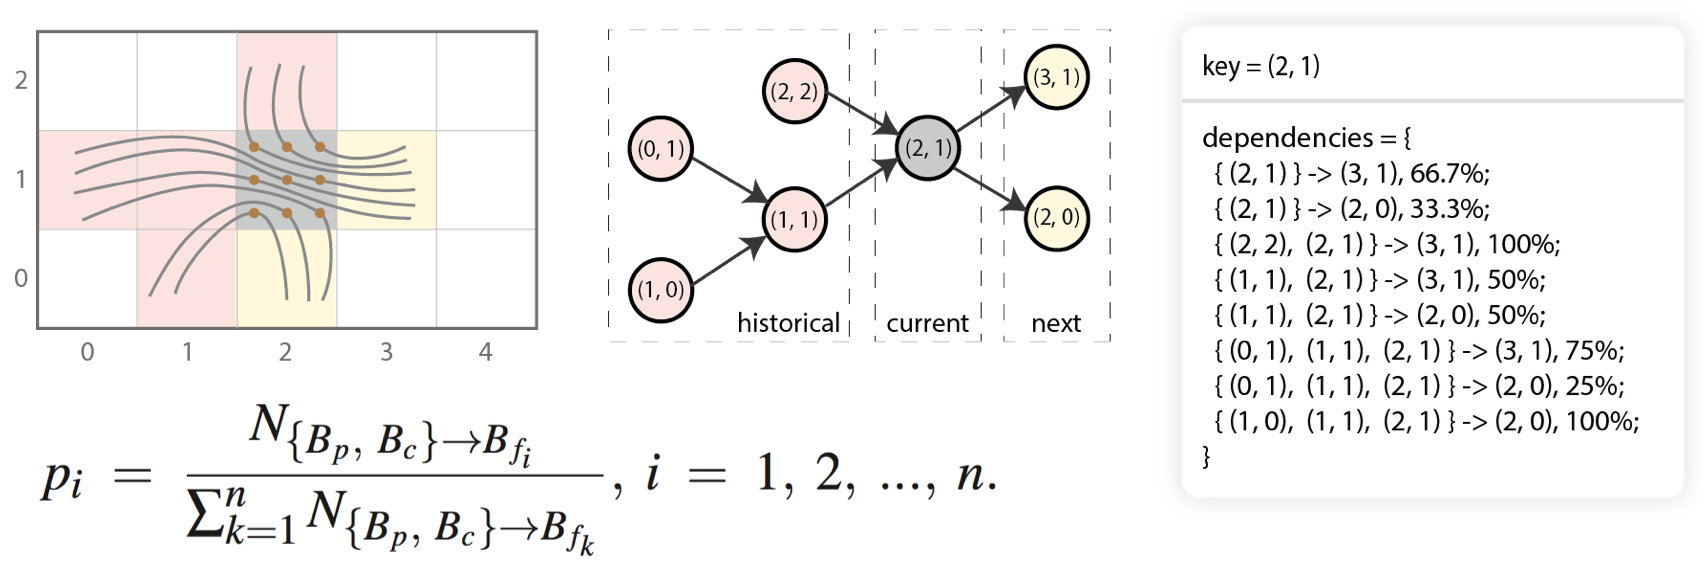
\includegraphics[width=\linewidth]{image/prefetch/highorder_fig3.png}
  \caption{
    高阶访问依赖的计算示意图。\parencite{ZhangGY16}
  }
  \label{fig:highorder_fig3}
\end{figure}


进一步将得到的高阶访问依赖应用到一个任务并行粒子追踪的框架中。数据块和其关联的高阶访问依赖是以数据项的形式进行存储。每个数据项包含三个部分:$<key, value, dependencies>$,分别表示数据块的时空索引、实际数据以及高阶访问依赖。在$dependencies$部分,对于具有相同历史访问信息的访问依赖,可以将它们重新组织,将其中下一步可能访问的数据块的$key$按照访问转移概率降序排列,这样$dependencies$里面可以看成是很多个键值对,方便之后的检索。

在运行时迹线计算过程中,使用了高阶数据预取来提高I/O效率。也就是说,当载入一个不在缓存中的数据项时,通过匹配粒子真实的历史数据访问信息和该数据项中高阶访问依赖的历史访问信息部分,得到具有最高转移概率的数据块并将其一并载入,以满足之后可能的数据访问需求。实际上,也可以通过设置预取深度来递归地预取多个深度的数据块,而在每个预取深度,也可以将多个高概率的数据块同时预取进来。图\ref{fig:highorder_fig4}展示了一个递归的预取过程。图中每个预取深度只取概率最大的数据块。

\begin{figure}[!tb]
  \centering
  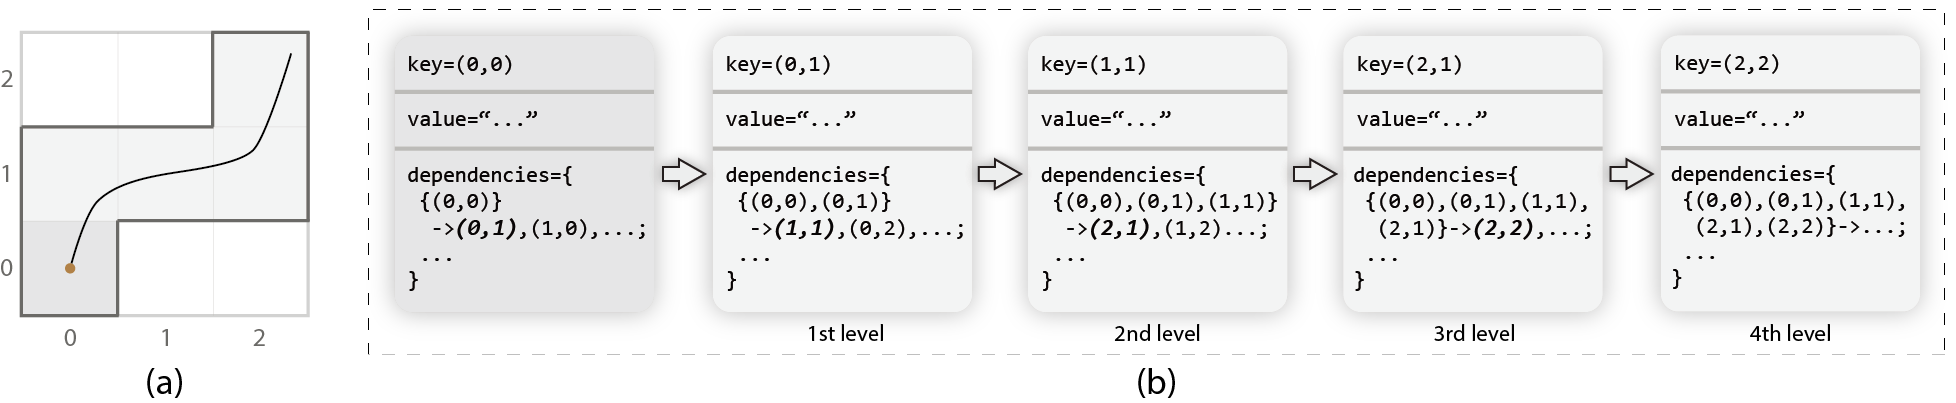
\includegraphics[width=\linewidth]{image/prefetch/highorder_fig4.png}
  \caption{
    一次性递归地预取多个数据项。\parencite{ZhangGY16}在这个例子中,预取深度设置为4,并且在每个预取深度 只预取概率最大的那个数据块。当请求块(0, 0)时,块(0, 1),(1, 1),(2, 1)和(2, 2)一个接一个地被预 测出来并被预取进内存。在每个预取深度,历史访问信息都会随之更新。
  }
  \label{fig:highorder_fig4}
\end{figure}


该方法仍然具有一定的局限性。首先是预处理开销,主要集中在迹线计算上,尽管采取了一定的策略,其代价仍然比较高,特别是对于大规模数据。因此,需要考虑更好的撒种策略。另外,合适参数的选择也是一个比较困难的问题,包括预取深度和数据块大小的设置等,虽然在该工作中都是经验指定的,但是各个参数和它们之间的联系仍然值得进一步地探究。

\subsection{深度学习支持的数据预取}
粒子追踪是流场可视化与分析里最重要的技术之一,被大量应用在场线渲染、源汇查询、有限时间李雅普诺夫指数计算等应用中。然而,在大规模流场中,对大量粒子通过粒子追踪算法计算轨迹时,由于粒子访问数据块的局部性很差,导致计算过程中有大量时间消耗在数据块的读入上。一种提高数据块访问效率的做法,就是对粒子将要访问的数据块进行预测,然后提前进行预读取,从而将读入花费隐藏在计算时间之下。这个工作\parencite{Hong2018LSTM}首次引入了深度学习模型,即基于长短期记忆 (Long Short-Term Memory, LSTM) 的模型,对粒子轨迹进行建模,从而能更为准确地预测粒子对数据块的访问,从而提高大规模粒子追踪算法的效率。

\begin{figure}[!tb]
  \centering
  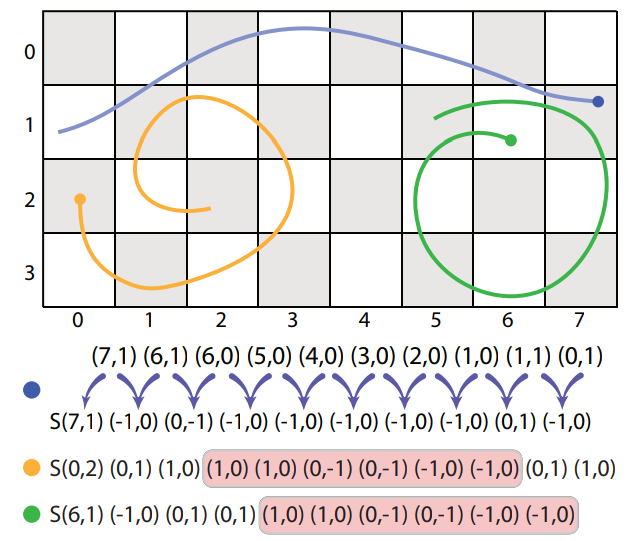
\includegraphics[width=.65\linewidth]{image/prefetch/lstm_fig1.png}
  \caption{
    粒子轨迹数据到移动序列数据的转换。\parencite{Hong2018LSTM}
  }
  \label{fig:lstm_fig1}
\end{figure}


为了将粒子轨迹转换为深度学习模型容易处理的数据,需要对其进行变换。首先,粒子轨迹的坐标序列被转化为粒子所访问数据块的序列。采用数据块而不是坐标,是已有数据预读取工作常用的做法,并且直接预测坐标容易在数据块边界附近出现错误。接下来,数据块序列被转换为相对移动的序列,即表现粒子如何在数据块之间穿行。图\ref{fig:lstm_fig1}中,以蓝色粒子为例,展示了这个转换过程,也就是相邻两个数据块的索引求差。为了保证转换后的移动序列和原本的数据块序列等价,在序列最前面加上粒子的初始数据块,并加上字母S区分。这样就完成了粒子轨迹数据的转换工作。这种转换的另一个好处是,深度学习的模型能学习到间接的访问模式。例如,图\ref{fig:lstm_fig1}中黄色、绿色粒子尽管初始数据块不同,但具有类似的旋转行为,因而在转换后的序列中具有相同的子序列。该模型能够学习到这种模式,并应用到其他粒子的行为预测中去,而已有的工作则不能。

\begin{figure}[!tb]
  \centering
  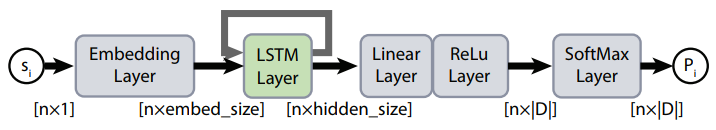
\includegraphics[width=.85\linewidth]{image/prefetch/lstm_fig2.png}
  \caption{
    基于LSTM实现的深度学习模型\parencite{Hong2018LSTM}
  }
  \label{fig:lstm_fig2}
\end{figure}

接下来,围绕LSTM构建深度学习模型,如图\ref{fig:lstm_fig2}所示。在这里,仅介绍模型的输入输出关系,细节部分请参阅论文以及相关深度学习资料。总起来看,该输入是粒子的移动序列$s_0, s_1, …, s_{n-1}$,其中$s_0$是粒子初始数据块索引。模型输出则是对应下一步移动的概率分布$P_0,P_1,…,P_{n-1}$。最初,模型接受$s_0$为输入,对粒子的第1步进行预测,得到其在各种移动可能性上的概率分布$P_0$。接着,模型又接受$s_1$为输入,对粒子的第2步进行预测,得到其在各种移动可能性上的概率分布$P_1$。需要注意地是,由于LSTM模型的性质,$s_0$也参与到了$P_1$的生成中。以此类推,粒子每一步移动的预测均由其之前所有访问的数据块序列来决定。

为了训练这个模型,从原始流场数据中采样一些较低精度的粒子轨迹,进行数据转换,作为训练集,选择超参数进行模型训练。文中对训练集大小以及超参数的选择与预测精度的关系进行了探索。

接着,将该预训练的模型部署在GPU上,为并行粒子追踪算法提供粒子数据块访问的预测功能。粒子追踪器通过提前的数据块预取,来提高运行效率。在该性能测试中,该工作选用了三个数据集:飓风伊莎贝尔、GEOS-5大气模拟和海洋模拟数据集。测试的布种策略为局部分析和全局分析,即在局部区域密集撒种,以及在整个空间域均匀撒种。在测试中,该方法与不带预取的方法以及使用高阶访问模式\parencite{ZhangGY16}进行预取的基准方法进行对比。

相比较于不带预取的方法,该方法有很大的性能提升。而相比较于使用高阶访问模式\parencite{ZhangGY16}进行预取的方法,该方法性能略高。在其他两个数据中也有类似的表现。而在全局分析中,相比较于不带预取的方法,该方法仍然具有很大的性能提升。而相比较于使用高阶访问模式\parencite{ZhangGY16}进行预取的方法,该方法性能略低一些。

需要注意的是,尽管该方法和高阶访问模式的方法性能基本接近,但该方法所需要的额外存储要远远小于高阶访问模式的存储,并且所需要的训练样本数目也更加少。例如对于飓风伊莎贝尔数据,该模型仅占用53MB,而4阶高阶访问依赖关系需要5.7GB,6阶更是需要20GB,比原数据更大。如果要求高阶访问依赖关系仅使用与该方法相同的额外存储空间,那么它的性能将会变得非常差。另一方面,该方法仅需要100多万的粒子进行训练,而高阶访问依赖关系要数倍于此。

总的来说,该工作首次采用了深度学习的技术来解决流场可视化中的粒子追踪问题。相比于已有工作,该方法方法能取得与已有方法相当的准确率和性能提升,并且只需要极小的额外存储和训练样本。

\subsection{基于其他I/O访问模式的数据预取}
除了上面提到的比较直接的数据块之间的访问依赖关系,一些更为复杂的I/O访问模式(包括空间模式、时间模式、模式重复次数和请求数据大小等)也可以被检测并提取出来。
Byna等人\parencite{BynaCSTG08}将这种I/O访问模式记录为I/O签名(signature),结合运行时真实的数据访问,用于在MPI-IO中提供数据预取的指导。
而当I/O访问模式非常随机或不可预测时,预测预取(speculative prefetching)往往可以比较可靠地确定随后的I/O访问。
预执行(pre-execution)技术就是一个很好的例子\parencite{ChenBSTG08},其可以重叠计算和I/O访问的过程,从而减小I/O的延迟,提高并行应用程序的I/O访问性能。
这些技术也适用于并行粒子跟踪,帮助提高其计算效率。

\subsection{小结}
数据预取是通过归纳已有的任务中的固有的数据特征来预测任务接下来会访问的数据内容。
% 大规模流场可视化中的粒子追踪算法很好地展现了流线的计算过程中对不同的数据的预取的巨大优势。
% 但是由于流线本身的特征复杂,我们借助不同的方法来对其进行探索。包括基于马尔可夫链等方法计算访问依赖或采用机器学习的方法计算一些隐式的规则。
% 这一系列工作表明,对复杂的科学数据中的数据预取是一种降低计算延迟的有效手段。
数据预取可以提高数据局部性,从而在粒子追踪中获得更高的I/O效率。
但是,为了获得精确的预取精度,经常需要对数据进行复杂的预处理,例如提取数据访问依赖等I/O模式,给并行粒子追踪计算带来了额外的开销。
不仅如此,这种预处理的复杂性往往和流场的规模和复杂性成正比,也限制了数据预取方法在大规模流场数据中的使用。
数据预取比较适合于在小型台式计算机\parencite{VermaKP00, ChenNLS12, ChenS13} 或者有限计算资源下的计算平台\parencite{GuoZLLYHMP14}上进行核外(out-of-core)方式的可视化应用。
